\chapter{Cheat sheet}
\label{chap:cheatsheet}

This chapter explains how to perform some common---and some not so
common---tasks in gretl's scripting language, hansl.  Some but not
all of the techniques listed here are also available through the
graphical interface.  Although the graphical interface may be more
intuitive and less intimidating at first, we encourage users to take
advantage of the power of gretl's scripting language as soon as
they feel comfortable with the program.

\section{Dataset handling}

\subsection{``Weird'' periodicities}

\emph{Problem:} You have data sampled each 3 minutes from 9am onwards;
you'll probably want to specify the hour as 20 periods.

\emph{Solution:}
\begin{code}
setobs 20 9:1 --special
\end{code}

\emph{Comment:} Now functions like \cmd{sdiff()} (``seasonal''
difference) or estimation methods like seasonal ARIMA will work as
expected.

\subsection{Generating a panel dataset of given dimensions}

\emph{Problem:} You want to generate via \cmd{nulldata} a panel
dataset and specify in advance the number of units and the time length
of your series via two scalar variables.

\emph{Solution:}
\begin{code}
scalar n_units = 100
scalar T = 12
scalar NT = T * n_units

nulldata NT --preserve
setobs T 1:1 --stacked-time-series
\end{code}

\emph{Comment:} The essential ingredient that we use here is the
\option{preserve} option: it protects existing scalars (and matrices,
for that matter) from being trashed by \cmd{nulldata}, thus making it
possible to use the scalar $T$ in the \cmd{setobs} command.

\subsection{Help, my data are backwards!}

\emph{Problem:} Gretl expects time series data to be in chronological
order (most recent observation last), but you have imported
third-party data that are in reverse order (most recent first).

\emph{Solution:}
\begin{code}
setobs 1 1 --cross-section
series sortkey = -obs
dataset sortby sortkey
setobs 1 1950 --time-series
\end{code}

\emph{Comment:} The first line is required only if the data currently
have a time series interpretation: it removes that interpretation,
because (for fairly obvious reasons) the \cmd{dataset sortby}
operation is not allowed for time series data.  The following two
lines reverse the data, using the negative of the built-in index
variable \texttt{obs}.  The last line is just illustrative: it
establishes the data as annual time series, starting in 1950.

If you have a dataset that is mostly the right way round, but a
particular variable is wrong, you can reverse that variable as
follows:
\begin{code}
x = sortby(-obs, x)
\end{code}


\subsection{Dropping missing observations selectively}

\emph{Problem:} You have a dataset with many variables and want to
restrict the sample to those observations for which there are no
missing observations for the variables \texttt{x1}, \texttt{x2} and
\texttt{x3}.

\begin{samepage}
\emph{Solution:}
\begin{code}
list X = x1 x2 x3
smpl --no-missing X
\end{code}
\end{samepage}

\emph{Comment:} You can save the file via a \cmd{store} command
to preserve a subsampled version of the dataset. Alternative solutions
based on the \cmd{ok} function, such as
\begin{code}
list X = x1 x2 x3
series sel = ok(X)
smpl sel --restrict
\end{code}
are perhaps less obvious, but more flexible. Pick your poison.

\subsection{``By'' operations}

\emph{Problem:} You have a discrete variable \texttt{d} and you want
to run some commands (for example, estimate a model) by splitting the
sample according to the values of \texttt{d}.

\emph{Solution:}
\begin{code}
matrix vd = values(d)
m = rows(vd)
loop i=1..m
  scalar sel = vd[i]
  smpl d==sel --restrict --replace
  ols y const x
endloop
smpl --full
\end{code}

\emph{Comment:} The main ingredient here is a loop.  You can have
gretl perform as many instructions as you want for each value of
\texttt{d}, as long as they are allowed inside a loop. Note, however,
that if all you want is descriptive statistics, the \cmd{summary}
command does have a \option{by} option.

\subsection{Adding a time series to a panel}

\emph{Problem:} You have a panel dataset (comprising observations of
$n$ indidivuals in each of $T$ periods) and you want to add a variable
which is available in straight time-series form.  For example, you
want to add annual CPI data to a panel in order to deflate nominal
income figures.

In gretl a panel is represented in stacked time-series format, so in
effect the task is to create a new variable which holds $n$ stacked
copies of the original time series.  Let's say the panel comprises 500
individuals observed in the years 1990, 1995 and 2000 ($n=500$,
$T=3$), and we have these CPI data in the ASCII file \texttt{cpi.txt}:

\begin{code}
date cpi
1990 130.658
1995 152.383
2000 172.192
\end{code}

What we need is for the CPI variable in the panel to repeat these
three values 500 times.

\emph{Solution:} Simple!  With the panel dataset open in gretl,
\begin{code}
append cpi.txt
\end{code}

\emph{Comment:} If the length of the time series is the same as the
length of the time dimension in the panel (3 in this example), gretl
will perform the stacking automatically.  Rather than using the
\cmd{append} command you could use the ``Append data'' item under
the \textsf{File} menu in the GUI program.

If the length of your time series does not exactly match the $T$
dimension of your panel dataset, \cmd{append} will not work but you
can use the \cmd{join} command, which is able to pick just the
observations with matching time periods. On selecting ``Append data''
in the GUI you are given a choice between plain ``append'' and
``join'' modes, and if you choose the latter you get a dialog window
allowing you to specify the key(s) for the join operation. For native
gretl data files you can use built-in series that identify the time
periods, such as \dollar{obsmajor}, for your outer key to match the
dates. In the example above, if the CPI data were in gretl format
\dollar{obsmajor} would give you the year of the observations.

\subsection{Time averaging of panel datasets}

\emph{Problem:} You have a panel dataset (comprising observations of
$n$ indidivuals in each of $T$ periods) and you want to lower the time
frequency by averaging. This is commonly done in empirical growth
economics, where annual data are turned into 3- or 4- or 5-year
averages \citep[see for example][]{Islam1995}.

\emph{Solution:} In a panel dataset, gretl functions that deal
with time are aware of the panel structure, so they will automatically
``do the right thing''. Therefore, all you have to do is use the
\cmd{movavg()} function for computing moving averages and then just
drop the years you don't need. An example with artificial data
follows:
\begin{code}
nulldata 36
set seed 61218
setobs 12 1:1 --stacked-time-series

###
### generate simulated yearly data
###
series year = 2000 + time
series y = round(normal())
series x = round(3*uniform())
list X = y x
print year X -o

###
### now re-cast as 4-year averages
###
# a dummy for endpoints
series endpoint = (year % 4 == 0)
# id variable
series id = $unit

# compute averages
loop foreach i X
    series $i = movavg($i, 4)
endloop

# drop extra observations
smpl endpoint --dummy --permanent

# restore panel structure
setobs id year --panel-vars
print id year X -o
\end{code}
% $
Running the above script produces (among other output):
\begin{code}
? print year X -o

             year            y            x

1:01         2001            1            1
1:02         2002           -1            1
1:03         2003           -1            0
1:04         2004            0            1
1:05         2005            1            2
1:06         2006            1            2
1:07         2007           -1            0
1:08         2008            1            1
1:09         2009            0            3
1:10         2010           -1            1
1:11         2011            1            1
1:12         2012            0            1
...
3:09         2009            0            1
3:10         2010            1            1
3:11         2011            0            2
3:12         2012            1            2

? print id year X -o

              id         year            y            x

1:1            1         2004        -0.25         0.75
1:2            1         2008         0.50         1.25
1:3            1         2012         0.00         1.50
...
3:3            3         2012         0.50         1.50
\end{code}

\subsection{Turning observation-marker strings into a series}

\emph{Problem:} Here's one that might turn up in the context of the
\cmd{join} command (see chapter~\ref{chap:join}). The current dataset
contains a string-valued series that you'd like to use as a key for
matching observations, perhaps the two-letter codes for the names of
US states. The file from which you wish to add data contains that same
information, but \textit{not} in the form of a string-valued series,
rather it exists in the form of ``observation markers''. Such markers
cannot be used as a key directly, but is there a way to parlay them
into a string-valued series? Why, of course there is!

\emph{Solution:}
We'll illustrate with the Ramanathan data file \texttt{data4-10.gdt},
which contains private school enrollment data and covariates for the
50 US states plus Washington, D.C. ($n = 51$).
\begin{code}
open data4-10.gdt
markers --to-array="state_codes"
genr index
stringify(index, state_codes)
store joindata.gdt
\end{code}

\emph{Comment:} The \texttt{markers} command saves the observation
markers to an array of strings. The command \texttt{genr index}
creates a series that goes 1, 2, 3, \dots{}, and we attach the state
codes to this series via \texttt{stringify()}. After saving the result
we have a datafile that contains a series, \texttt{index}, that can be
matched with whatever series holds the state code strings in the
target dataset.

Suppose the relevant string-valued key series in the target dataset is
called \texttt{state}. We might prefer to avoid the need to specify a
distinct ``outer'' key (again see chapter~\ref{chap:join}). In that
case, in place of
\begin{code}
genr index
stringify(index, state_codes)
\end{code}
we could do
\begin{code}
genr index
series state = index
stringify(state, state_codes)
\end{code}
and the two datafiles will contain a comparable string-valued
\texttt{state} series.

\section{Creating/modifying variables}

\subsection{Generating a dummy variable for a specific observation}

\emph{Problem:} Generate $d_t = 0$ for all observations but one, for
which $d_t = 1$.

\emph{Solution:}
\begin{code}
  series d = (t=="1984:2")
\end{code}

\emph{Comment:} The internal variable \texttt{t} is used to refer to
observations in string form, so if you have a cross-section sample you
may just use \texttt{d = (t=="123")}. If the dataset has observation
labels you can use the corresponding label, in which case it's more
idiomatic to use \texttt{obs} rather than \texttt{t}. For example, if
you open the dataset \texttt{mrw.gdt}, supplied with gretl among the
examples, a dummy variable for Italy could be generated via
\begin{code}
  series DIta = (obs=="Italy")
\end{code}

Note that this method does not require scripting. You can use the GUI
menu itrm ``Add/Define new variable'' for the same purpose, with the
same syntax.

\subsection{Generating a discrete variable out of a set of dummies}

\emph{Problem:} The \cmd{dummify} function (also available as a
command) generates a set of mutually exclusive dummies from a discrete
variable. The reverse functionality, however, seems to be absent.

\emph{Solution:}
\begin{code}
series x = lincomb(D, seq(1, nelem(D)))
\end{code}

\emph{Comment:} Suppose you have a list \texttt{D} of mutually
exclusive dummies, that is a full set of 0/1 variables coding for the
value of some characteristic, such that the sum of the values of the
elements of \texttt{D} is 1 at each observation. This is, by the way,
exactly what the \cmd{dummify} command produces.  The reverse job of
\cmd{dummify} can be performed neatly by using the \cmd{lincomb}
function.

The code above multiplies the first dummy variable in the list
\texttt{D} by 1, the second one by 2, and so on. Hence, the return
value is a series whose value is $i$ if and only if the $i$-th member
of \texttt{D} has value 1.

If you want your coding to start from 0 instead of 1, you'll have to
modify the code snippet above into
\begin{code}
series x = lincomb(D, seq(0, nelem(D)-1))
\end{code}

\subsection{Easter}

\emph{Problem:} I have a 7-day daily dataset. How do I create an
``Easter'' dummy?

\emph{Solution:} We have the \cmd{easterday()} function, which returns
the month and day of Easter (in the form of a single scalar that must
be unpacked) given the year. The following example script uses this
function and a few string magic tricks. It assumes a 7-day dataset
that spans at least 2011 to 2016.

\begin{code}
series Easter = 0
loop y=2011..2016
    a = easterday(y)
    m = floor(a)
    d = round(100*(a-m))
    ed_str = sprintf("%04d-%02d-%02d", y, m, d)
    Easter["@ed_str"] = 1
endloop
\end{code}

\emph{Comment:} The \cmd{round()} function is necessary for the
``day'' component because otherwise floating-point problems may
ensue. Try the year 2015, for example.

\subsection{Recoding a variable}

\emph{Problem:} You want to perform a 1-to-1 recode on a variable. For
example, consider tennis points: you may have a variable $x$ holding
values 1 to 3 and you want to recode it to 15, 30, 40.

\emph{Solution 1:}
\begin{code}
series x = replace(x, 1, 15)
series x = replace(x, 2, 30)
series x = replace(x, 3, 40)
\end{code}

\emph{Solution 2:}
\begin{code}
matrix tennis = {15, 30, 40}
series x = replace(x, seq(1,3), tennis)
\end{code}

\emph{Comment:} There are many equivalent ways to achieve the same
effect, but for simple cases such as this, the \cmd{replace} function
is simple and transparent. If you don't mind using matrices, scripts
using \cmd{replace} can also be remarkably compact. Note that
\cmd{replace} also performs $n$-to-1 (``surjective'') replacements,
such as
\begin{code}
series x = replace{z, {2, 3, 5, 11, 22, 33}, 1)
\end{code}
which would turn all entries equal to 2, 3, 5, 11, 22 or 33 to 1 and
leave the other ones unchanged.

\subsection{Generating a ``subset of values'' dummy}

\emph{Problem:} You have a dataset which contains a fine-grained
coding for some qualitative variable and you want to ``collapse'' this
to a relatively small set of dummy variables. Examples: you have place
of work by US state and you want a small set of regional dummies; or
you have detailed occupational codes from a census dataset and you
want a manageable number of occupational category dummies.

Let's call the source series \texttt{src} and one of the target dummies
\texttt{D1}. And let's say that the values of \texttt{src} to be grouped
under \texttt{D1} are 2, 13, 14 and 25. We'll consider three possible
solutions: ``Longhand,'' ``Clever,'' and ``Proper.''

\emph{``Longhand'' solution:}
\begin{code}
series D1 = src==2 || src==13 || src==14 || src==25
\end{code}

\emph{Comment:} The above works fine if the number of distinct values
in the source to be condensed into each dummy variable is fairly
small, but it becomes cumbersome if a single dummy must comprise
dozens of source values.

\emph{Clever solution:}
\begin{code}
matrix sel = {2,13,14,25}
series D1 = maxr({src} .= vec(sel)') .> 0
\end{code}

\emph{Comment:} The subset of values to be grouped together can be
written out as a matrix relatively compactly (first line). The magic
that turns this into the desired series (second line) relies on the
versatility of the ``dot'' (element-wise) matrix operators. The
expression ``\texttt{\{src\}}'' gets a column-vector version of the
input series---call this $x$---and ``\texttt{vec(sel)'}'' gets the
input matrix as a row vector, in case it's a column vector or a matrix
with both dimensions greater than 1---call this $s$. If $x$ is
$n\times1$ and $s$ is $1\times m$, the ``\texttt{.=}'' operator
produces an $n\times m$ result, each element $(i,j)$ of which equals 1
if $x_i = s_j$, otherwise 0. The \texttt{maxr()} function along with
the ``\verb|.>|'' operator (see chapter~\ref{chap:matrices} for both)
then produces the result we want.

Of course, whichever procedure you use, you have to repeat for each of
the dummy series you want to create (but keep reading---the ``proper''
solution is probably what you want if you plan to create several
dummies).

\emph{Further comment:} Note that the clever solution depends on
converting what is ``naturally'' a vector result into a series. This
will fail if there are missing values in \texttt{src}, since (by
default) missing values will be skipped when converting \texttt{src}
to $x$, and so the number of rows in the result will fall short of the
number of observations in the dataset. One fix is then to subsample
the dataset to exclude missing values before employing this method;
another is to adjust the \dtk{skip_missing} setting via the
\cmd{set} command (see the \GCR).

\emph{Proper solution:}

The best solution, in terms of both computational efficiency and code
clarity, would be using a ``conversion table'' and the \cmd{replace}
function, to produce a series on which the \cmd{dummify} command can
be used. For example, suppose we want to convert from a series called
\texttt{fips} holding FIPS codes\footnote{FIPS is the Federal
  Information Processing Standard: it assigns numeric codes from 1 to
  56 to the US states and outlying areas.} for the 50 US states plus
the District of Columbia to a series holding codes for the four
standard US regions. We could create a $2 \times 51$ matrix---call it
\texttt{srmap}---with the 51 FIPS codes on the first row and the
corresponding region codes on the second, and then do
\begin{code}
series region = replace(fips, srmap[1,], srmap[2,])
\end{code}

\subsection{Generating an ARMA(1,1)}

\emph{Problem:} Generate $y_t = 0.9 y_{t-1} + \varepsilon_t - 0.5
\varepsilon_{t-1}$, with $\varepsilon_t \sim N\!I\!I\!D(0,1)$.

\emph{Recommended solution:}
\begin{code}
alpha = 0.9
theta = -0.5
series y = filter(normal(), {1, theta}, alpha)
\end{code}

\emph{``Bread and butter'' solution:}
\begin{code}
alpha = 0.9
theta = -0.5
series e = normal()
series y = 0
series y = alpha * y(-1) + e + theta * e(-1)
\end{code}

\emph{Comment:} The \cmd{filter} function is specifically designed for
this purpose so in most cases you'll want to take advantage of its
speed and flexibility. That said, in some cases you may want to
generate the series in a manner which is more transparent (maybe for
teaching purposes).

In the second solution, the statement \cmd{series y = 0} is necessary
because the next statement evaluates \texttt{y} recursively, so
\texttt{y[1]} must be set.  Note that you must use the keyword
\texttt{series} here instead of writing \texttt{genr y = 0} or simply
\texttt{y = 0}, to ensure that \texttt{y} is a series and
not a scalar.

\subsection{Recoding a variable by classes}

\emph{Problem:} You want to recode a variable by classes. For example,
you have the age of a sample of individuals ($x_i$) and you need to
compute age classes ($y_i$) as
\begin{eqnarray*}
  y_i = 1 & \mathrm{for} & x_i < 18 \\
  y_i = 2 & \mathrm{for} & 18 \le x_i < 65 \\
  y_i = 3 & \mathrm{for} & x_i \ge 65
\end{eqnarray*}

\emph{Solution:}
\begin{code}
series y = 1 + (x >= 18) + (x >= 65)
\end{code}

\emph{Comment:} True and false expressions are evaluated as 1 and 0
respectively, so they can be manipulated algebraically as any other
number. The same result could also be achieved by using the
conditional assignment operator (see below), but in most cases it
would probably lead to more convoluted constructs.

\subsection{Conditional assignment}

\emph{Problem:} Generate $y_t$ via the following rule:
\[
  y_t = \left\{
    \begin{array}{ll}
      x_t & \mathrm{for} \quad d_t > a \\
      z_t & \mathrm{for} \quad d_t \le a
    \end{array}
    \right.
\]

\emph{Solution:}
\begin{code}
series y = (d > a) ? x : z
\end{code}

\emph{Comment:} There are several alternatives to the one presented
above. One is a brute force solution using loops. Another one, more
efficient but still suboptimal, would be
\begin{code}
series y = (d>a)*x + (d<=a)*z
\end{code}
However, the ternary conditional assignment operator is not only the
most efficient way to accomplish what we want, it is also remarkably
transparent to read when one gets used to it. Some readers may find it
helpful to note that the conditional assignment operator works exactly
the same way as the \texttt{=IF()} function in spreadsheets.

\subsection{Generating a time index for panel datasets}

\emph{Problem:} gretl has a \texttt{\$unit} accessor, but not
the equivalent for time. What should I use?

\emph{Solution:}
\begin{code}
series x = time
\end{code}

\emph{Comment:} The special construct \cmd{genr time} and its variants
are aware of whether a dataset is a panel.

\subsection{Sanitizing a list of regressors}

\emph{Problem:} I noticed that built-in commands like \cmd{ols}
automatically drop collinear variables and put the constant first. How
can I achieve the same result for an estimator I'm writing?

\emph{Solution:}
No worry. The function below does just that
\begin{code}
function list sanitize(list X)
    list R = X - const
    if nelem(R) < nelem(X)
        R = const R
    endif
    return dropcoll(R)
end function
\end{code}
so for example the code below
\begin{code}
nulldata 20
x = normal()
y = normal()
z = x + y # collinear
list A = x y const z
list B = sanitize(A)

list print A
list print B
\end{code}
returns
\begin{code}
? list print A
x y const z
? list print B
const x y
\end{code}

Aside: it has been brought to our attention that some mischievous
programs out there put the constant \emph{last}, instead of first,
like God intended. We are not amused by this utter disrespect of
econometric tradition, but if you want to pursue the way of evil, it
is rather simple to adapt the script above to that effect.


\subsection{Generating the ``hat'' values after an OLS regression}
\label{sec:hatvalues}

\emph{Problem:} I've just run an OLS regression, and now I need the
so-called the leverage values (also known as the ``hat'' values). I
know you can access residuals and fitted values through ``dollar''
accessors, but nothing like that seems to be available for ``hat''
values.

\emph{Solution:}
``Hat'' values are can be thought of as the diagonal of the projection
matrix $P_X$, or more explicitly as
\[
h_i = \mathbf{x}_i' (X'X)^{-1} \mathbf{x}_i
\]
where $X$ is the matrix of regressors and $\mathbf{x}_i'$ is its
$i$-th row.

The reader is invited to study the code below, which offers four
different solutions to the problem:

\begin{code}
open data4-1.gdt --quiet
list X = const sqft bedrms baths
ols price X

# method 1
leverage --save --quiet
series h1 = lever

# these are necessary for what comes next
matrix mX  = {X}
matrix iXX = invpd(mX'mX)

# method 2
series h2 = diag(qform(mX, iXX))
# method 3
series h3 = sumr(mX .* (mX*iXX))
# method 4
series h4 = NA
loop i=1..$nobs
    matrix x = mX[i,]'
    h4[i] = x'iXX*x
endloop

# verify
print h1 h2 h3 h4 --byobs
\end{code}
%$

\emph{Comment:} Solution 1 is the preferable one: it relies on the
built-in \cmd{leverage} command, which computes the requested series
quite efficiently, taking care of missing values, possible
restrictions to the sample, etc.

However, three more are shown for didactical purposes, mainly to show
the user how to manipulate matrices. Solution 2 first constructs the
$P_X$ matrix explicitly, via the \cmd{qform} function, and then takes
its diagonal; this is definitely \emph{not} recommended (despite its
compactness), since you generate a much bigger matrix than you
actually need and waste a lot of memory and CPU cycles in the
process. It doesn't matter very much in the present case, since the
sample size is very small, but with a big dataset this could be a very
bad idea.

Solution 3 is more clever, and relies on the fact that, if you
define $Z = X\cdot(X'X)^{-1}$, then $h_i$ could also
be written as
\[
 h_i = \mathbf{x}_i' \mathbf{z}_i = \sum_{i=1}^k x_{ik} z_{i_k}
\]
which is in turn equivalent to the sum of the elements of the $i$-th
row of $X \odot Z$, where $\odot$ is the element-by-element
product. In this case, your clever usage of matrix algebra would
produce a solution computationally much superior to solution 2.

Solution 4 is the most old-fashioned one, and employs an indexed
loop. While this wastes practically no memory and employs no more CPU
cycles in algebraic operations than strictly necessary, it imposes a
much greater burden on the hansl interpreter, since handling a loop is
conceptually more complex than a single operation. In practice, you'll
find that for any realistically-sized problem, solution 4 is much
slower that solution 3.

\subsection{Moving functions for time series}
\label{sec:movfun}

\emph{Problem:} gretl provides native functions for moving
averages, but I need a to compute a different statistic on a sliding
data window. Is there a way to do this without using loops?

\emph{Solution:} One of the nice things of the \texttt{list} data type
is that, if you define a list, then several functions that would
normally apply ``vertically'' to elements of a series apply
``horizontally'' across the list. So for example, the following piece
of code
\begin{code}
open bjg.gdt
order = 12
list L = lg || lags(order-1, lg)
smpl +order ;
series movmin = min(L)
series movmax = max(L)
series movmed = median(L)
smpl full
\end{code}
computes the moving minimum, maximum and median of the \texttt{lg}
series. Plotting the four series would produce something similar to
figure \ref{fig:movfun}.

\begin{figure}[hbtp]
  \centering
  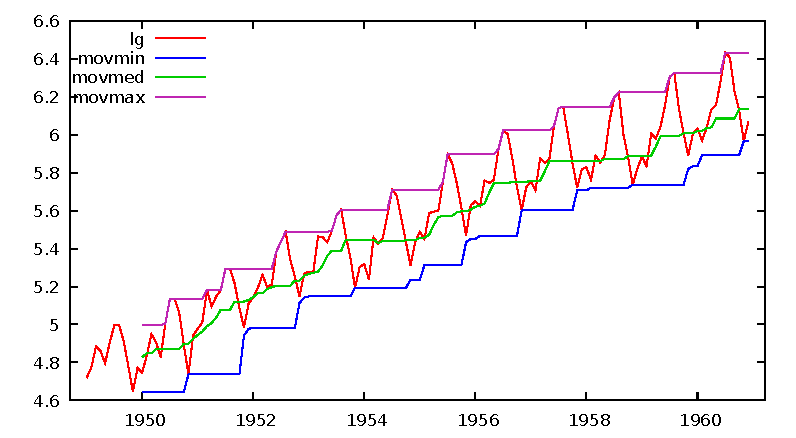
\includegraphics{figures/movfun}
  \caption{``Moving'' functions}
  \label{fig:movfun}
\end{figure}

\subsection{Generating data with a prescribed correlation structure}
\label{sec:CholeskyTrick}

\emph{Problem:} I'd like to generate a bunch of normal random variates
whose covariance matrix is exactly equal to a given matrix
$\Sigma$. How can I do this in gretl?

\emph{Solution:} The Cholesky decomposition is your friend. If you
want to generate data with a given \emph{population} covariance
matrix, then all you have to do is post-multiply your pseudo-random
data by the Cholesky factor (transposed) of the matrix you want. For
example:
\begin{code}
set seed 123
S = {2,1;1,1}
T = 1000
X = mnormal(T, rows(S))
X = X * cholesky(S)'
eval mcov(X)
\end{code}
should give you
\begin{code}
? eval mcov(X)
      2.0016       1.0157
      1.0157       1.0306
\end{code}

If, instead, you want your simulated data to have a given \emph{sample}
covariance matrix, you have to apply the same technique twice: one for
standardizing the data, another one for giving it the covariance
structure you want. Example:
\begin{code}
S = {2,1;1,1}
T = 1000
X = mnormal(T, rows(S))
X = X * (cholesky(S)/cholesky(mcov(X)))'
eval mcov(X)
\end{code}
gives you
\begin{code}
? eval mcov(X)
   2   1
   1   1
\end{code}
as required.

\section{Neat tricks}
\label{sec:cheat-neat}

\subsection{Interaction dummies}

\emph{Problem:} You want to estimate the model $y_i = \mathbf{x}_i
\beta_1 + \mathbf{z}_i \beta_2 + d_i \beta_3 + (d_i \cdot \mathbf{z}_i)
\beta_4 + \varepsilon_t$, where $d_i$ is a dummy variable while
$\mathbf{x}_i$ and $\mathbf{z}_i$ are vectors of explanatory
variables.

\emph{Solution:} As of version 1.9.12, gretl provides the
\verb|^| operator to make this operation easy. See section
\ref{sec:transform-lists} for details (especially
Listing~\ref{ex:interaction-lists}). But back in my day,
we used loops to do that! Here's how:

\begin{code}
list X = x1 x2 x3
list Z = z1 z2
list dZ = deflist()
loop foreach i Z
  series d$i = d * $i
  list dZ = dZ d$i
endloop

ols y X Z d dZ
\end{code}
%$

\emph{Comment:} It's amazing what string substitution can do for
you, isn't it?

\subsection{Realized volatility}

\emph{Problem:} Given data by the minute, you want to compute the
``realized volatility'' for the hour as $RV_t = \frac{1}{60}
\sum_{\tau=1}^{60} y_{t:\tau}^2$. Imagine your sample starts at time 1:1.

\emph{Solution:}
\begin{code}
smpl --full
genr time
series minute = int(time/60) + 1
series second = time % 60
setobs minute second --panel
series rv = psd(y)^2
setobs 1 1
smpl second==1 --restrict
store foo rv
\end{code}

\emph{Comment:} Here we trick gretl into thinking that our
dataset is a panel dataset, where the minutes are the ``units'' and
the seconds are the ``time''; this way, we can take advantage of the
special function \cmd{psd()}, panel standard deviation.  Then we
simply drop all observations but one per minute and save the resulting
data (\texttt{store foo rv} translates as ``store in the gretl
datafile \texttt{foo.gdt} the series \texttt{rv}'').

\subsection{Looping over two paired lists}

\emph{Problem:} Suppose you have two lists with the same number of
elements, and you want to apply some command to corresponding elements
over a loop. For example you want to regress each element of one
list on the corresponding element of the other.

\emph{Solution:}
\begin{code}
list Y = y1 y2 y3
list X = x1 x2 x3
loop i=1..nelem(Y)
   ols Y[i] 0 X[i]
endloop
\end{code}

\subsection{Convolution / polynomial multiplication}

\emph{Problem:} How do I multiply polynomials? There's no dedicated
function to do that, and yet it's a fairly basic mathematical task.

\emph{Solution:} Never fear! We have the \cmd{conv2d} function, which
is a tool for a more general problem, but includes polynomial
multiplication as a special case..

Suppose you want to multiply two finite-order polynomials $P(x) =
\sum_{i=0}^m p_i x^i$ and $Q(x) = \sum_{i=0}^n q_i x^i$. What you want
is the sequence of coefficients of the polynomial
\[
  R(x) = P(x) \cdot Q(x) = \sum_{k=0}^{m+n} r_k x^k
\]
where
\[
  r_k = \sum_{i=0}^k p_i q_{k-i}
\]
is the \emph{convolution} of the $p_i$ and $q_i$ coefficients. The
same operation can be performed via the FFT, but in most cases using
\cmd{conv2d} is quicker and more natural.

As an example, we'll use the same one we used in Section
\ref{sec:genr-fft}: consider the multiplication of two polynomials:
\begin{eqnarray*}
  P(x) & = & 1 + 0.5 x \\
  Q(x) & = & 1 + 0.3 x - 0.8 x^2 \\
  R(x) = P(x) \cdot Q(x) & = & 1 + 0.8 x - 0.65 x^2 - 0.4 x^3
\end{eqnarray*}
The following code snippet performs all the necessary calculations:
\begin{code}
p = {1; 0.5}
q = {1; 0.3; -0.8}
r = conv2d(p, q)
print r
\end{code}
Runnning the above produces
\begin{code}
r (4 x 1)

      1
    0.8
  -0.65
   -0.4
\end{code}
which is indeed the desired result. Note that the same computation
could also be performed via the \cmd{filter} function, at the price of
slightly more elaborate syntax.

\subsection{Comparing two lists}

\emph{Problem:} How can I tell if two lists contain the same variables
(not necessarily in the same order)?

\emph{Solution:} In many respects, lists are like sets, so it makes
sense to use the so-called ``symmetric difference'' operator, which is
defined as
\[
A\,\triangle\,B = (A \setminus B) \cup (B \setminus A)
\]
where in this context backslash represents the relative complement
operator, which gives the elements of set $A$ than are not in set $B$:
\[
A \setminus B = \left\{ x \in A : x \not \in B \right\}
\]
So we first check if there are any series in $A$ but not in $B$, then
we perform the reverse check. If the union of the two results is an
empty set, then the lists must contain the same variables. The hansl
syntax for this would be something like
\begin{code}
scalar NotTheSame = nelem((A-B) || (B-A)) > 0
\end{code}

\subsection{Reordering list elements}

\emph{Problem:} Is there a way to reorder list elements?

\emph{Solution:} You can use the fact that a list can be cast into
a vector of integers and then manipulated via ordinary matrix
syntax. So, for example, if you wanted to ``flip'' a list you may
just use the \cmd{mreverse} function. For example:
\begin{code}
open AWM.gdt --quiet
list X = 3 6 9 12
matrix tmp = X
list revX = mreverse(tmp')

list X print
list revX print
\end{code}
will produce
\begin{code}
? list X print
D1 D872 EEN_DIS GCD
? list revX print
GCD EEN_DIS D872 D1
\end{code}

\subsection{Plotting an asymmetric confidence interval}

\emph{Problem:} ``I like the look of the \option{band} option to the
\cmd{gnuplot} and \cmd{plot} commands, but it's set up for plotting a
symmetric interval and I want to show an asymmetric one.''

\emph{Solution:} Any interval is by construction symmetrical about its
mean at each observation. So you just need to perform a little
tweak. Say you want to plot a series \texttt{x} along with a band
defined by the two series \texttt{top} and \texttt{bot}. Here we go:
\begin{code}
# create series for mid-point and deviation
series mid = (top + bot)/2
series dev = top - mid
gnuplot x --band=mid,dev --time-series --with-lines --output=display
\end{code}

\subsection{Cross-validation}
\label{sec:xvalid}

\emph{Problem:} ``I'd like to compute the so-called \emph{leave-one-out
cross-validation criterion} for my regression. Is there a command in
gretl?''

If you have a sample with $n$ observations, the ``leave-one-out''
cross-validation criterion can be mechanically computed by running $n$
regressions in which one observation at a time is omitted and all the
other ones are used to forecast its value. The sum of the $n$ squared
forecast errors is the statistic we want. Fortunately, there is no
need to do so. It is possible to prove that the same statistic can be
computed as
\[
CV = \sum_{i=1}^n [\hat{u}_{i}/(1-h_{i})]^2,
\]
where $h_i$ is the $i$-th element of the ``hat'' matrix (see section
\ref{sec:hatvalues}) from a regression on the whole sample.

This method is natively provided by gretl as a side benefit to the
\cmd{leverage} command, that stores the CV criterion into the
\dollar{test} accessor. The following script shows the equivalence of
the two approaches:
\begin{code}
set verbose off
open data4-1.gdt
list X = const sqft bedrms baths

# compute the CV criterion the silly way

scalar CV = 0
matrix mX = {X}
loop i = 1 .. $nobs
    xi = mX[i,]
    yi = price[i]
    smpl obs != i --restrict
    ols price X --quiet
    smpl full
    scalar fe = yi - xi * $coeff
    CV += fe^2
endloop

printf "CV = %g\n", CV

# the smart way

ols price X --quiet
leverage --quiet
printf "CV = %g\n", $test
\end{code}

\subsection{Is my matrix result broken?}
\label{sec:brokenmat}

\emph{Problem:} Most of the matrix manipulation functions available
in gretl flag an error if something goes wrong, but there's no
guarantee that every matrix computation will return an entirely finite
matrix, containing no infinities or \texttt{NaN}s. So how do I tell if
I've got a fully valid matrix?

\emph{Solution}: The \texttt{sum} function applied to a matrix
\texttt{m} returns the sum of all of its elements or \texttt{NA} if
any elements are non-finite. So ``\texttt{eval sum(m)}'' can be used
as a check---or more explicitly,
\begin{code}
if !ok(sum(m))
    print "m is broken"
endif
\end{code}
Also note that the call ``\texttt{ok(m)}'' returns a matrix with the
same dimensions as \texttt{m}, with elements 1 for finite values and 0
for infinities or \texttt{NaN}s.

%%% Local Variables:
%%% mode: latex
%%% TeX-master: "gretl-guide"
%%% End:
